% ===== linear-regression =====
\section*{Linear Regression}

\subsection*{What Linear Regression Does}
\begin{itemize}
  \item Self-driving car: input $\mathbf{x}$ = image of the road, output = steering direction.
  \item This is \textbf{supervised learning}: we get labeled pairs $(\mathbf{x}, t)$.
\end{itemize}

\subsection*{Running Example: House Prices}
Start by collecting a dataset of houses and their prices:

\begin{center}
\begin{tabular}{cc}
\toprule
Size (ft$^2$) & Price (\$1000s) \\
\midrule
2104 & 400 \\
1416 & 232 \\
1534 & 315 \\
852  & 178 \\
\vdots & \vdots \\
\bottomrule
\end{tabular}
\end{center}

Or plot size vs.\ price and fit a straight line through the points.

{\centering
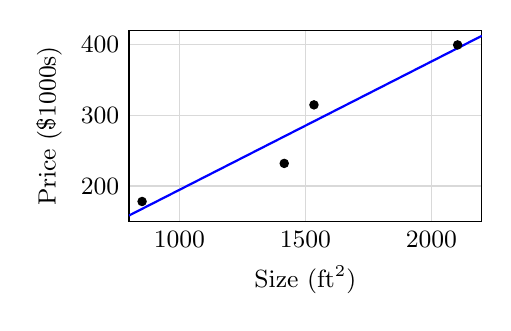
\begin{tikzpicture}
\begin{axis}[
    width=0.5\linewidth, height=4cm,
    xmin=800, xmax=2200, ymin=150, ymax=420,
    enlargelimits=false,
    grid=major, grid style={gray!30},
    major tick length=0pt,
    xlabel={Size (ft$^2$)}, ylabel={Price (\$1000s)},
    tick label style={font=\small}, label style={font=\small},
    xticklabel style={/pgf/number format/1000 sep={}}
]
\addplot[only marks, mark=*, mark size=1.5pt] coordinates {
    (2104,400) (1416,232) (1534,315) (852,178)
};
\addplot[thick, blue, domain=800:2200, samples=2] {12.5 + 0.182*x};
\end{axis}
\end{tikzpicture}
\par}

\subsection*{The Supervised Learning Pipeline}
\[
\text{Training set } \mathcal{D} \;\longrightarrow\; \text{Learning algorithm} \;\longrightarrow\; \text{Hypothesis } y(\mathbf{x}, \mathbf{w})
\]
The learning algorithm turns the training set into a function (the \textbf{hypothesis}), which takes a house we haven't seen and outputs an estimated price.

\subsection*{Representing the Hypothesis}
One feature ($x_1$ = size):
\[
y(\mathbf{x}, \mathbf{w}) = w_0 + w_1 x_1
\]

Two features: add number of bedrooms.

\begin{center}
\begin{tabular}{ccc}
\toprule
Size $x_1$ & \# Bedrooms $x_2$ & Price $t$ \\
\midrule
2104 & 3 & 400 \\
1416 & 2 & 232 \\
1534 & 3 & 315 \\
852  & 2 & 178 \\
\bottomrule
\end{tabular}
\end{center}

\[
y(\mathbf{x}, \mathbf{w}) = w_0 + w_1 x_1 + w_2 x_2
\]

\textbf{Dummy feature trick:} define $x_0 = 1$ always, so the bias $w_0$ has a feature to multiply and fits inside one dot product $\mathbf{w}^\top\mathbf{x}$. Then
\[
y(\mathbf{x}, \mathbf{w}) = \sum_{d=0}^{D} w_d x_d = \mathbf{w}^\top \mathbf{x},
\qquad
\mathbf{x} = \begin{bmatrix} 1 \\ x_1 \\ x_2 \end{bmatrix},\;
\mathbf{w} = \begin{bmatrix} w_0 \\ w_1 \\ w_2 \end{bmatrix}
\]
Example: $\mathbf{w} = [50,\, 0.1,\, 20]^\top$, house $(2104, 3)$:
$\mathbf{w}^\top\mathbf{x} = 50(1) + 0.1(2104) + 20(3) = 320.4$.

\subsection*{The Loss (Least Squares / OLS)}
\[
E(\mathbf{w}) = \frac{1}{2}\sum_{n=1}^{N} \Big( \underbrace{y(\mathbf{x}_n, \mathbf{w})}_{\text{prediction}} - \underbrace{t_n}_{\text{target}} \Big)^2
\]
This is the squared difference between prediction and target, summed over all $N$ examples. The $\tfrac12$ only cancels the 2 when differentiating; it doesn't change the minimizer.

We want the weights that minimize the loss, $\mathbf{w}^* = \arg\min_{\mathbf{w}} E(\mathbf{w})$. Two ways to find them: solve directly (\textbf{normal equation}) or iterate (\textbf{gradient descent}).

\subsection*{Normal Equation (Closed Form)}
For linear regression we can \textbf{jump straight to the minimum}: the bottom of the bowl has zero slope, so set the gradient to $\mathbf{0}$ and solve directly.

{\centering
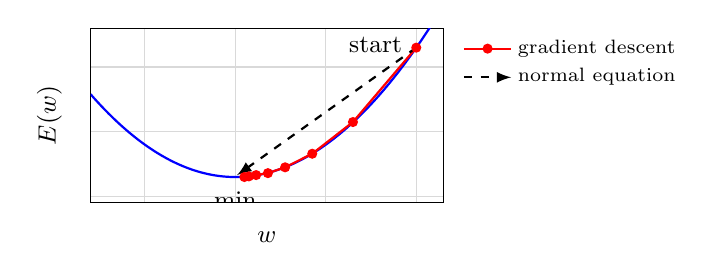
\begin{tikzpicture}
\begin{axis}[
    width=0.5\linewidth, height=3.8cm,
    xmin=-1.6, xmax=2.3, ymin=-0.1, ymax=2.6,
    enlargelimits=false,
    grid=major, grid style={gray!30}, major tick length=0pt,
    xlabel={$w$}, ylabel={$E(w)$},
    tick label style={font=\small}, label style={font=\small},
    xticklabels={}, yticklabels={},
    legend pos=outer north east, legend style={font=\scriptsize, draw=none}
]
\addplot[thick, blue, domain=-1.6:2.3, samples=100, forget plot] {0.5*x^2 + 0.3};
\addplot[red, thick, mark=*, mark size=1.4pt] coordinates {
    (2.00,2.30) (1.30,1.15) (0.85,0.66) (0.55,0.45) (0.36,0.36) (0.23,0.33) (0.15,0.31) (0.10,0.30)
};
\addlegendentry{gradient descent}
\addplot[black, thick, dashed, -latex] coordinates {(2.00,2.30) (0.02,0.33)};
\addlegendentry{normal equation}
\node[font=\small, anchor=east] at (axis cs:1.95,2.35) {start};
\node[font=\small, anchor=north] at (axis cs:0,0.22) {min};
\end{axis}
\end{tikzpicture}
\par}

\subsection*{Deriving the Normal Equation}

\textbf{Step 1: Rewrite the loss in matrix form.}
\[
\mathbb{X} = \begin{bmatrix} \mathbf{x}_1^\top \\ \vdots \\ \mathbf{x}_N^\top \end{bmatrix} \in \mathbb{R}^{N\times(D+1)},
\qquad
\mathbf{t} = \begin{bmatrix} t_1 \\ \vdots \\ t_N \end{bmatrix} \in \mathbb{R}^{N}
\]
\begin{itemize}
  \item $\mathbb{X}$: the \textbf{design matrix}, one row per example (including the dummy 1).
  \item $\mathbf{t}$: all the targets.
  \item $\mathbb{X}\mathbf{w}$: all $N$ predictions at once. $\;\mathbb{X}\mathbf{w} - \mathbf{t}$: all $N$ errors (prediction minus target).
\end{itemize}

The loss is half the sum of squared errors, and a vector dotted with itself is the sum of its squares, so:
\[
E(\mathbf{w}) = \frac12\sum_{n=1}^{N}\big(y(\mathbf{x}_n,\mathbf{w}) - t_n\big)^2 = \frac12(\mathbb{X}\mathbf{w} - \mathbf{t})^\top(\mathbb{X}\mathbf{w} - \mathbf{t})
\]

\textbf{Step 2: Set the gradient to zero and solve for $\mathbf{w}$.}
\begin{align*}
E(\mathbf{w})
&= \frac12\big(\mathbf{w}^\top\mathbb{X}^\top\mathbb{X}\mathbf{w} - 2\,\mathbf{w}^\top\mathbb{X}^\top\mathbf{t} + \mathbf{t}^\top\mathbf{t}\big)
  \qquad \text{(expand like $(a-b)^2 = a^2 - 2ab + b^2$)} \\
\nabla_{\mathbf{w}} E
&= \mathbb{X}^\top\mathbb{X}\mathbf{w} - \mathbb{X}^\top\mathbf{t}
  \qquad \text{(using $\nabla_{\mathbf{w}}\, \mathbf{w}^\top A\mathbf{w} = 2A\mathbf{w}$ and $\nabla_{\mathbf{w}}\, \mathbf{w}^\top\mathbf{u} = \mathbf{u}$)} \\
\mathbf{0}
&= \mathbb{X}^\top\mathbb{X}\mathbf{w} - \mathbb{X}^\top\mathbf{t}
  \qquad \text{(set the gradient to zero)}
\end{align*}
\begin{itemize}
  \item Expanding: the two middle terms $\mathbf{w}^\top\mathbb{X}^\top\mathbf{t}$ and $\mathbf{t}^\top\mathbb{X}\mathbf{w}$ are the same single number, so they combine into $-2\,\mathbf{w}^\top\mathbb{X}^\top\mathbf{t}$.
  \item Gradient: $A = \mathbb{X}^\top\mathbb{X}$ and $\mathbf{u} = \mathbb{X}^\top\mathbf{t}$; $\mathbf{t}^\top\mathbf{t}$ has no $\mathbf{w}$, so it drops. These are the matrix versions of $\tfrac{d}{dw}aw^2 = 2aw$ and $\tfrac{d}{dw}uw = u$.
\end{itemize}
Rearranging gives the \textbf{normal equation} $\mathbb{X}^\top\mathbb{X}\,\mathbf{w} = \mathbb{X}^\top\mathbf{t}$. Multiply both sides by $(\mathbb{X}^\top\mathbb{X})^{-1}$ (the matrix version of dividing):
\[
\mathbf{w}^* = (\mathbb{X}^\top\mathbb{X})^{-1}\mathbb{X}^\top\mathbf{t}
\]

\begin{itemize}
  \item \textbf{Requires $\mathbb{X}^\top\mathbb{X}$ to be invertible.} Fails if $N < D+1$ (fewer examples than weights) or if features are redundant. Fix: ridge regression, $\mathbf{w}^* = (\mathbb{X}^\top\mathbb{X} + \lambda I)^{-1}\mathbb{X}^\top\mathbf{t}$.
  \item \textbf{Normal equation vs.\ gradient descent.} The normal equation is exact and takes one step, but the inverse is expensive for large problems and it only works for linear regression.
  \item \textbf{Geometric view.} $\mathbb{X}\mathbf{w}^*$ is the closest point to $\mathbf{t}$ reachable by the columns of $\mathbb{X}$, so the error is perpendicular to every column: $\mathbb{X}^\top(\mathbb{X}\mathbf{w}^* - \mathbf{t}) = \mathbf{0}$.
\end{itemize}
